\section{Evaluation}

%%%%%%%%%%%%%%%%%%%%%%%%%%%%%%%%%%%%%%%%%%%%%%

\subsection{Query I/O}

\begin{figure}[ht]
\centerline{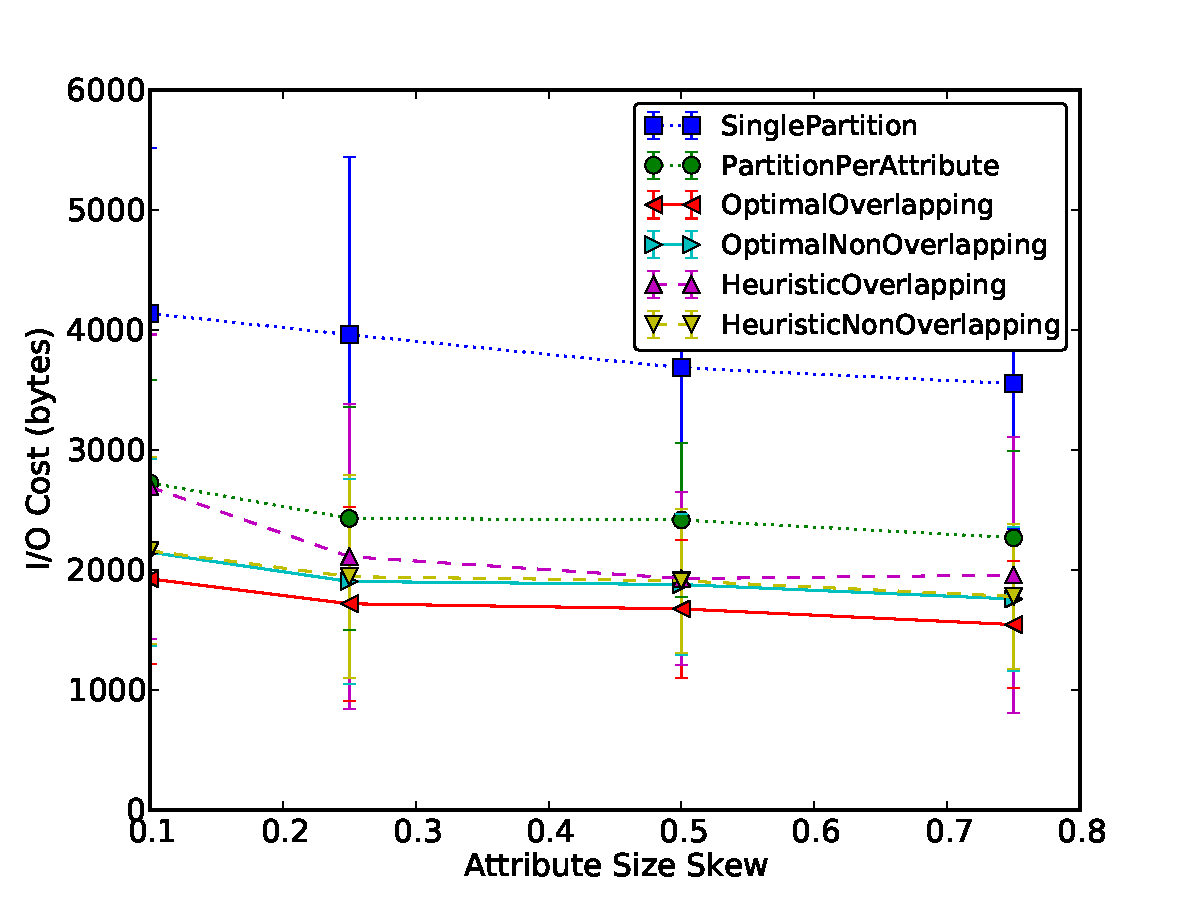
\includegraphics[width=0.9\columnwidth]{figures/QueryIOVsAttributeSizeSkew.pdf}}
\caption{QueryIOVsAttributeSizeSkew}
\end{figure}

\begin{figure}[ht]
\centerline{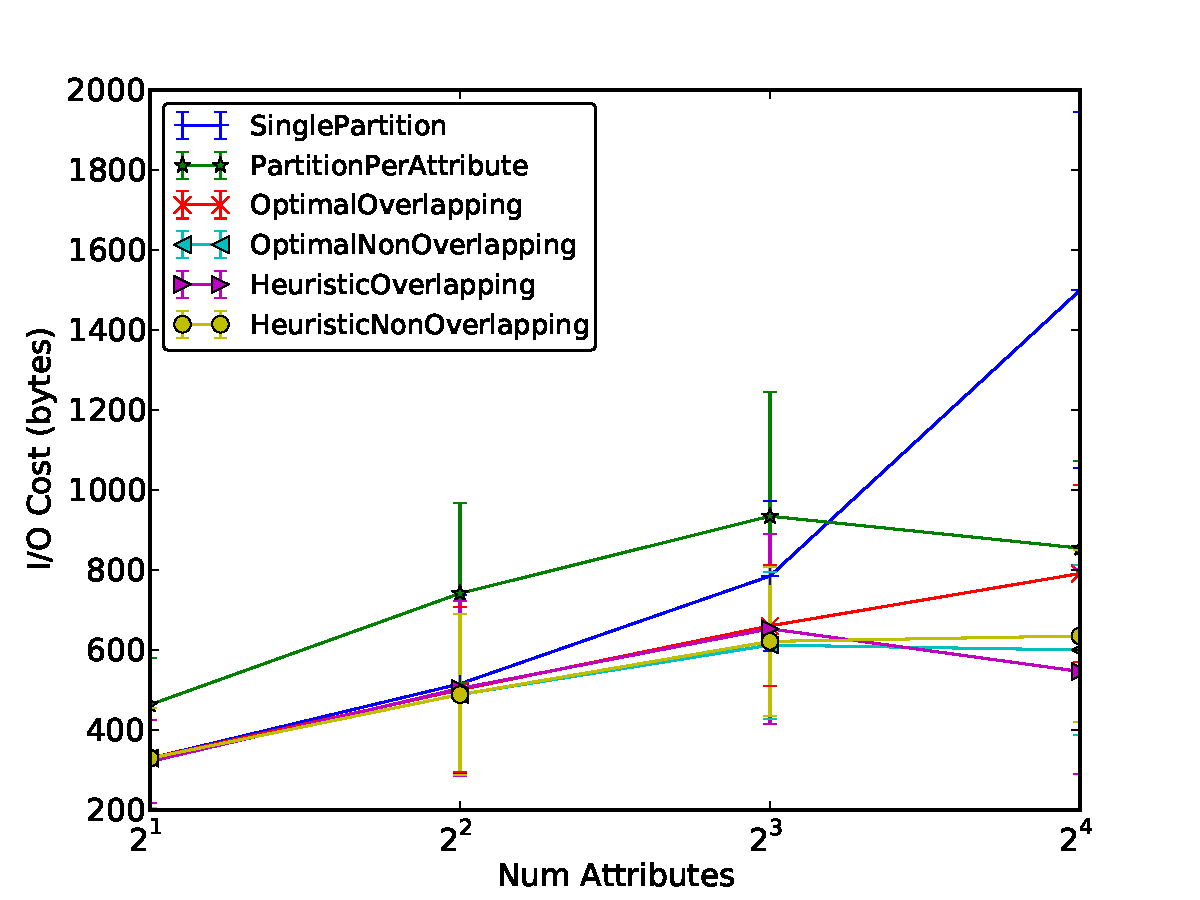
\includegraphics[width=0.9\columnwidth]{figures/QueryIOVsNumAttributes.pdf}}
 \caption{QueryIOVsNumAttributes}
 \end{figure}

\begin{figure}[ht]
\centerline{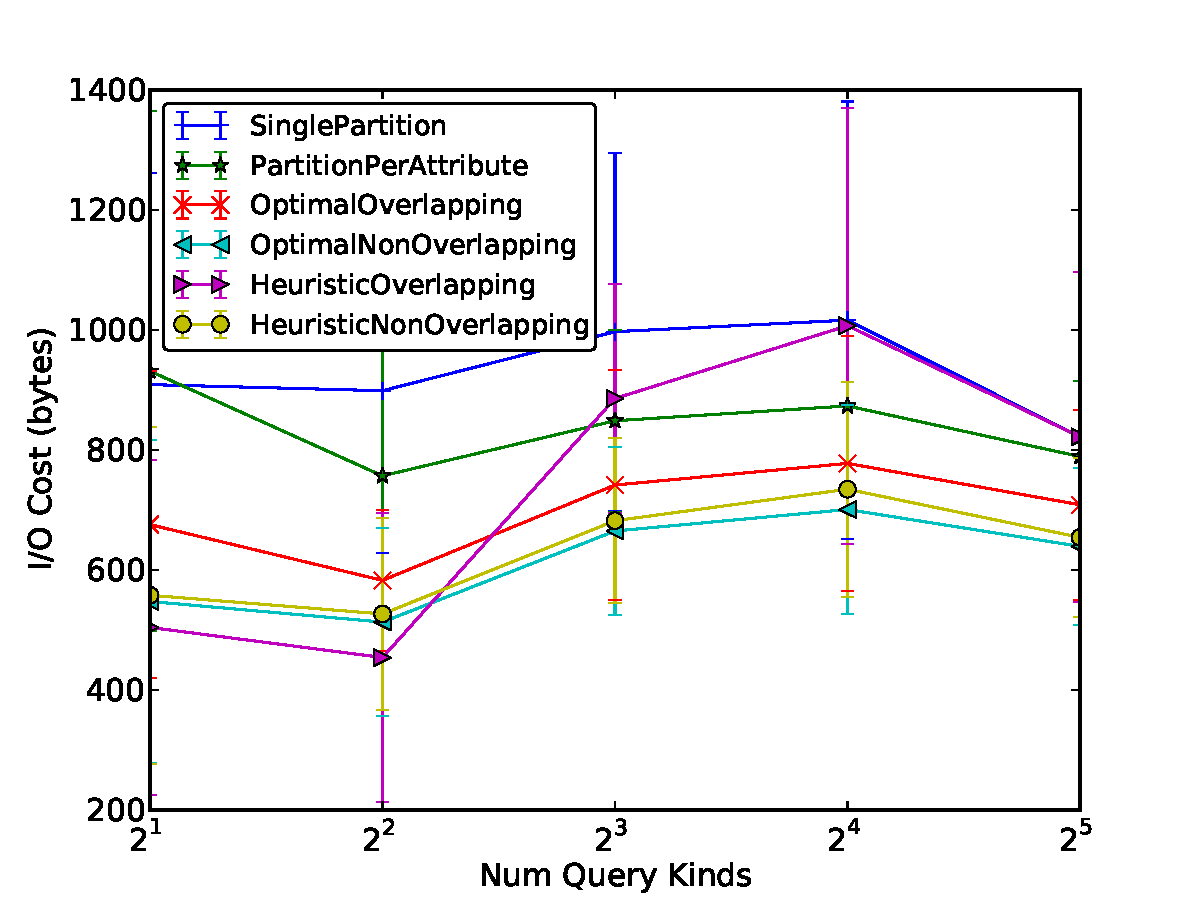
\includegraphics[width=0.9\columnwidth]{figures/QueryIOVsNumQueryKinds.pdf}}
\caption{QueryIOVsNumQueryKinds}
\end{figure}

\begin{figure}[ht]
 \centerline{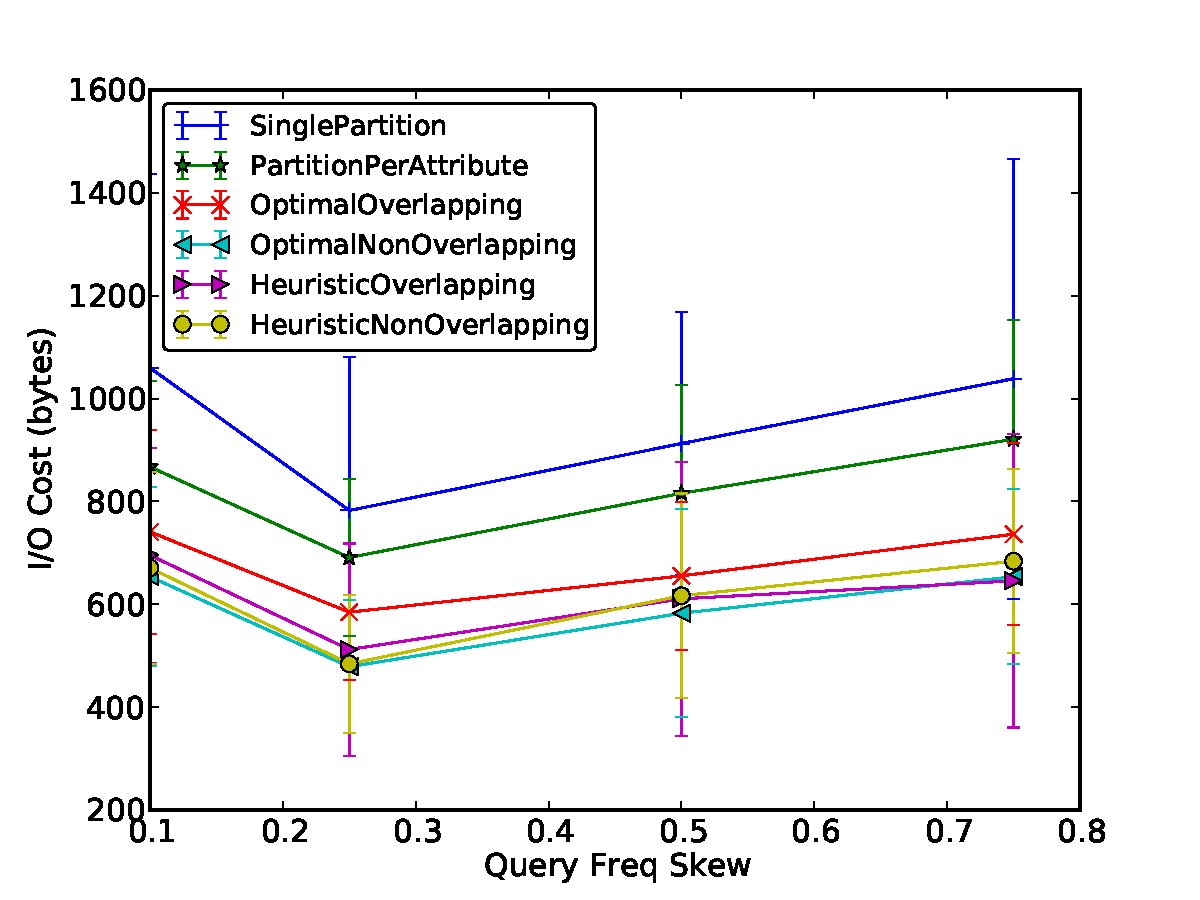
\includegraphics[width=0.9\columnwidth]{figures/QueryIOVsQueryFreqSkew.pdf}}
 \caption{QueryIOVsQueryFreqSkew}
 \end{figure}

 \begin{figure}[ht]
 \centerline{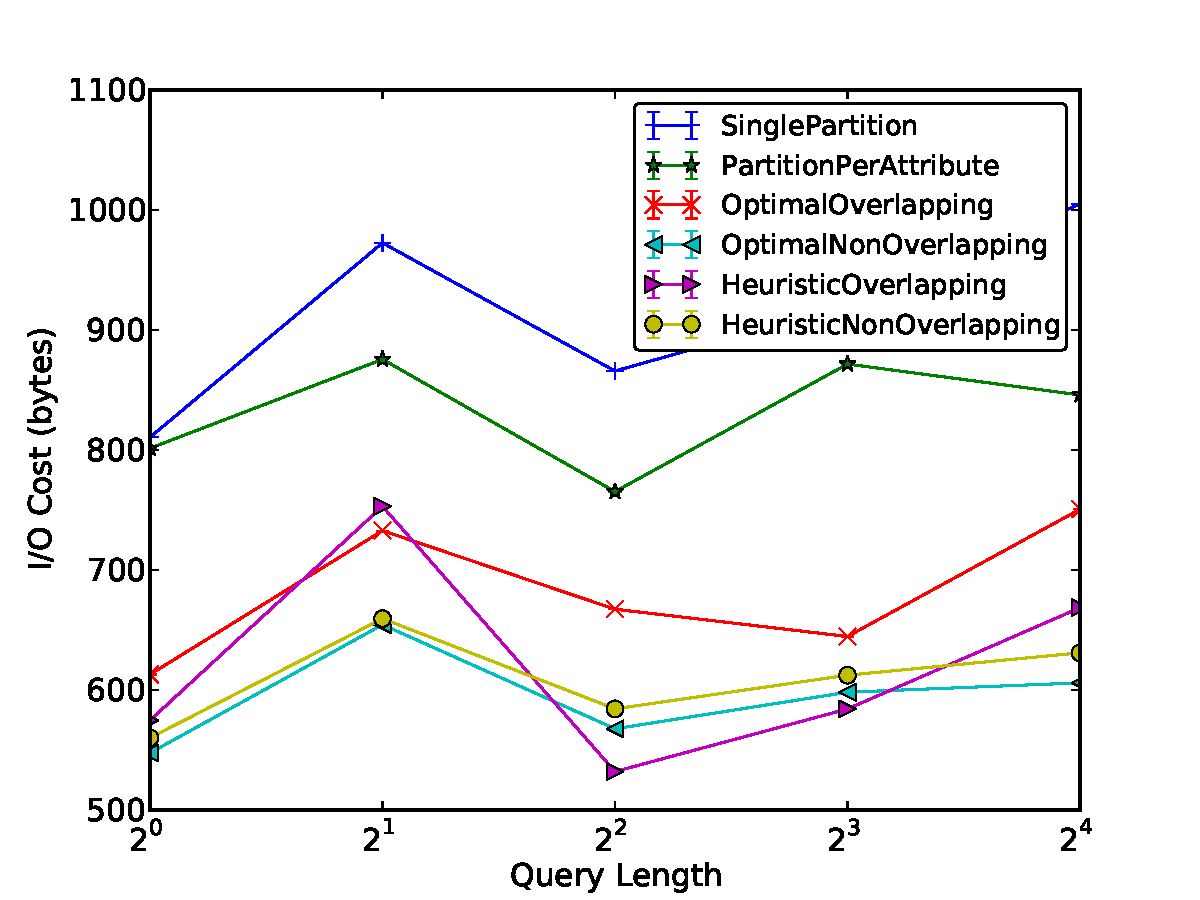
\includegraphics[width=0.9\columnwidth]{figures/QueryIOVsQueryLength.pdf}}
 \caption{QueryIOVsQueryLength}
 \end{figure}

 \begin{figure}[ht]
 \centerline{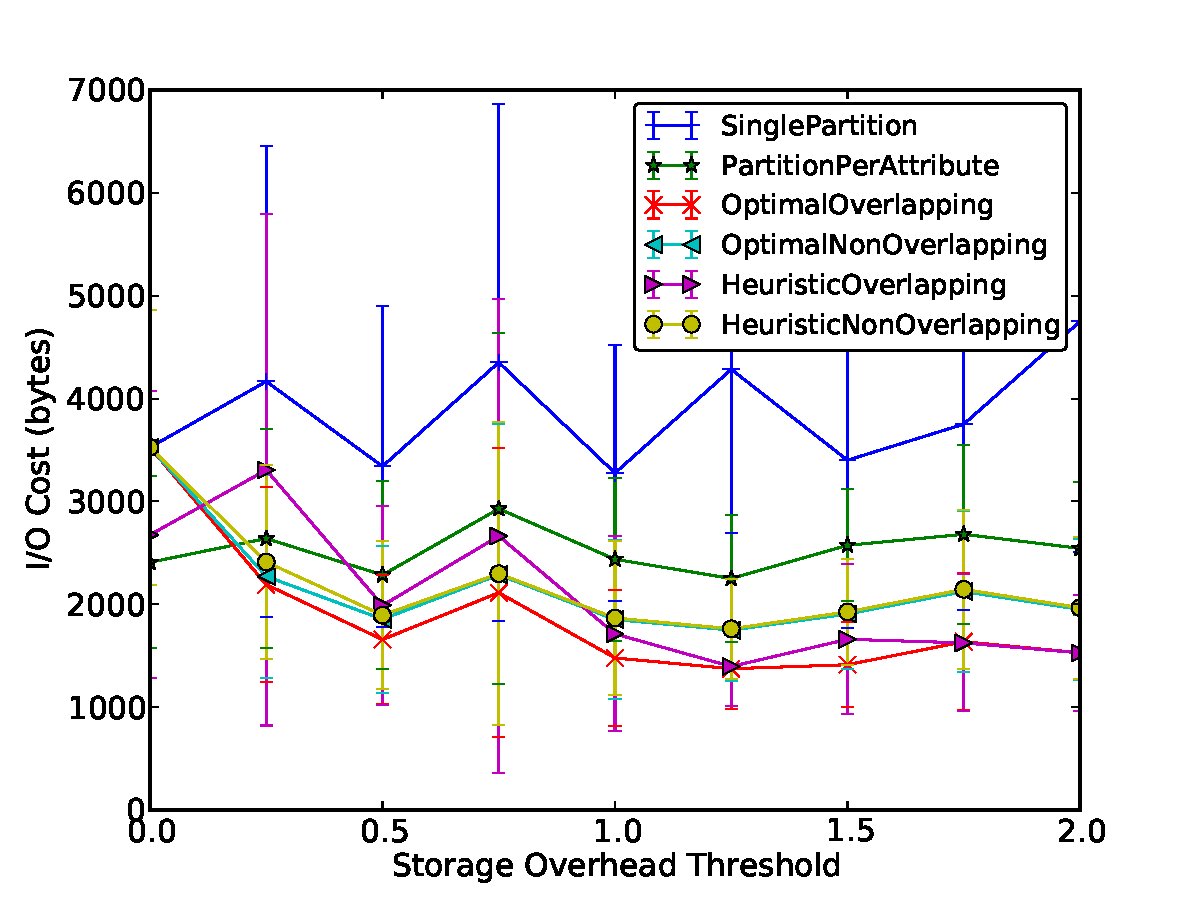
\includegraphics[width=0.9\columnwidth]{figures/QueryIOVsStorageOverheadThreshold.pdf}}
 \caption{QueryIOVsStorageOverheadThreshold}
 \end{figure}

% %%%%%%%%%%%%%%%%%%%%%%%%%%%%%%%%%%%%%%%%%%%%%%

\subsection{Running Time}

\begin{figure}[ht]
\centerline{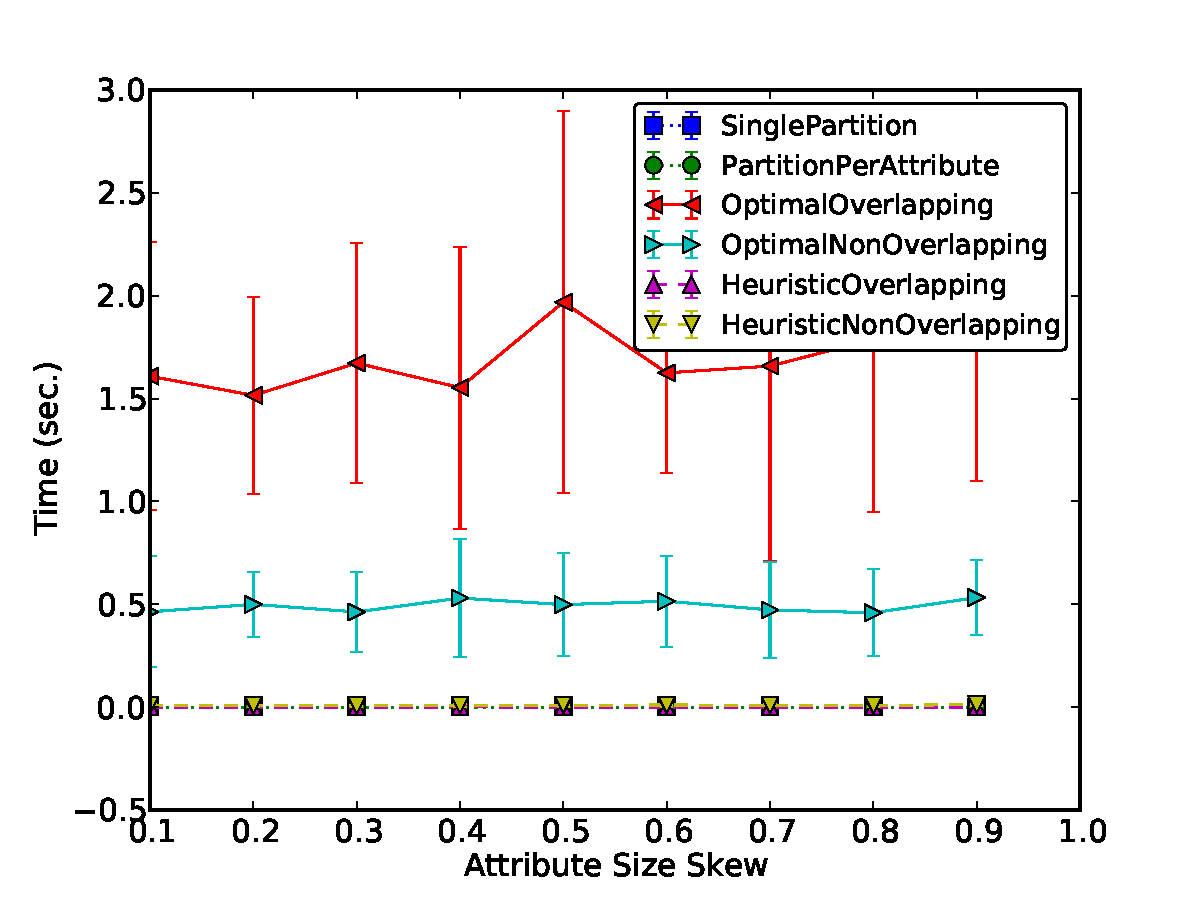
\includegraphics[width=0.9\columnwidth]{figures/RunningTimeVsAttributeSizeSkew.pdf}}
\caption{RunningTimeVsAttributeSizeSkew}
\end{figure}

\begin{figure}[ht]
\centerline{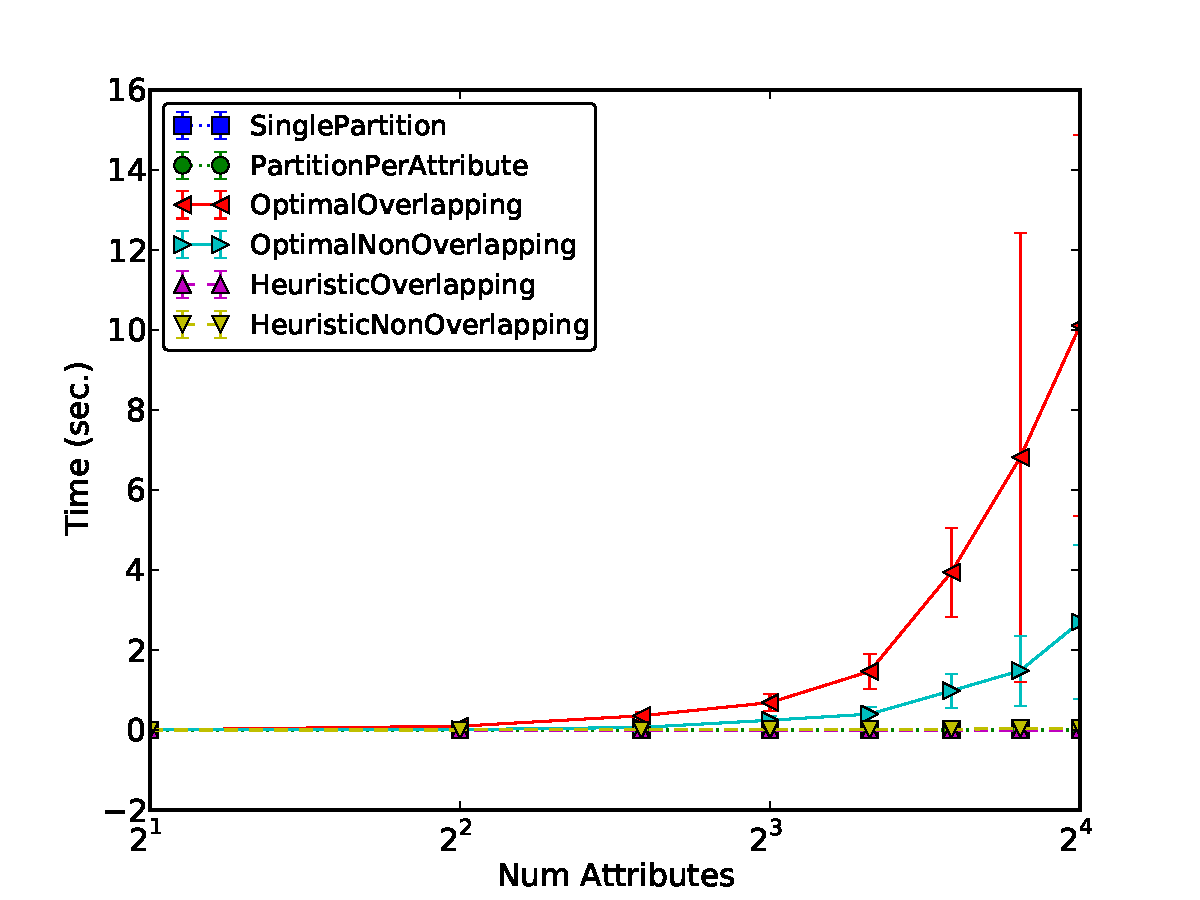
\includegraphics[width=0.9\columnwidth]{figures/RunningTimeVsNumAttributes.pdf}}
\caption{RunningTimeVsNumAttributes}
\end{figure}

\begin{figure}[ht]
\centerline{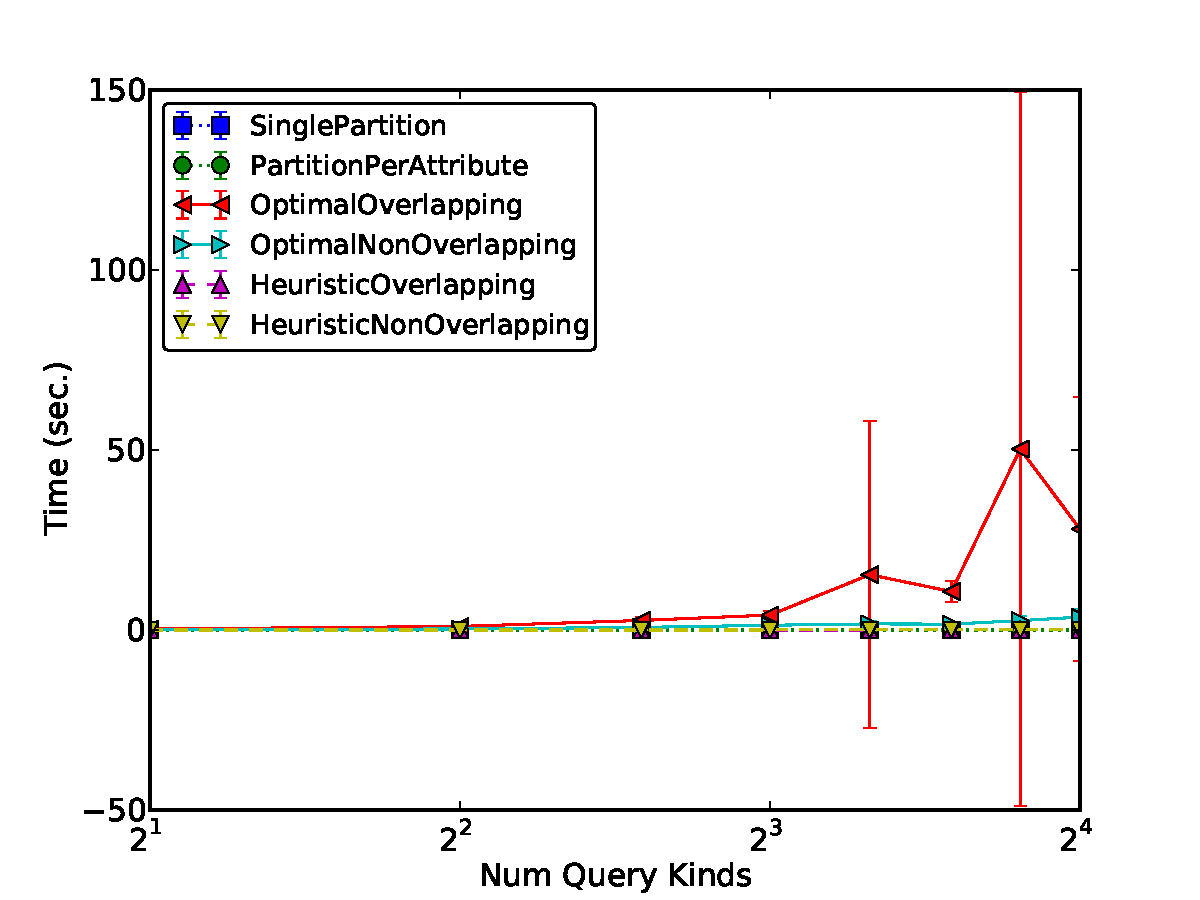
\includegraphics[width=0.9\columnwidth]{figures/RunningTimeVsNumQueryKinds.pdf}}
\caption{RunningTimeVsNumQueryKinds}
\end{figure}

\begin{figure}[ht]
\centerline{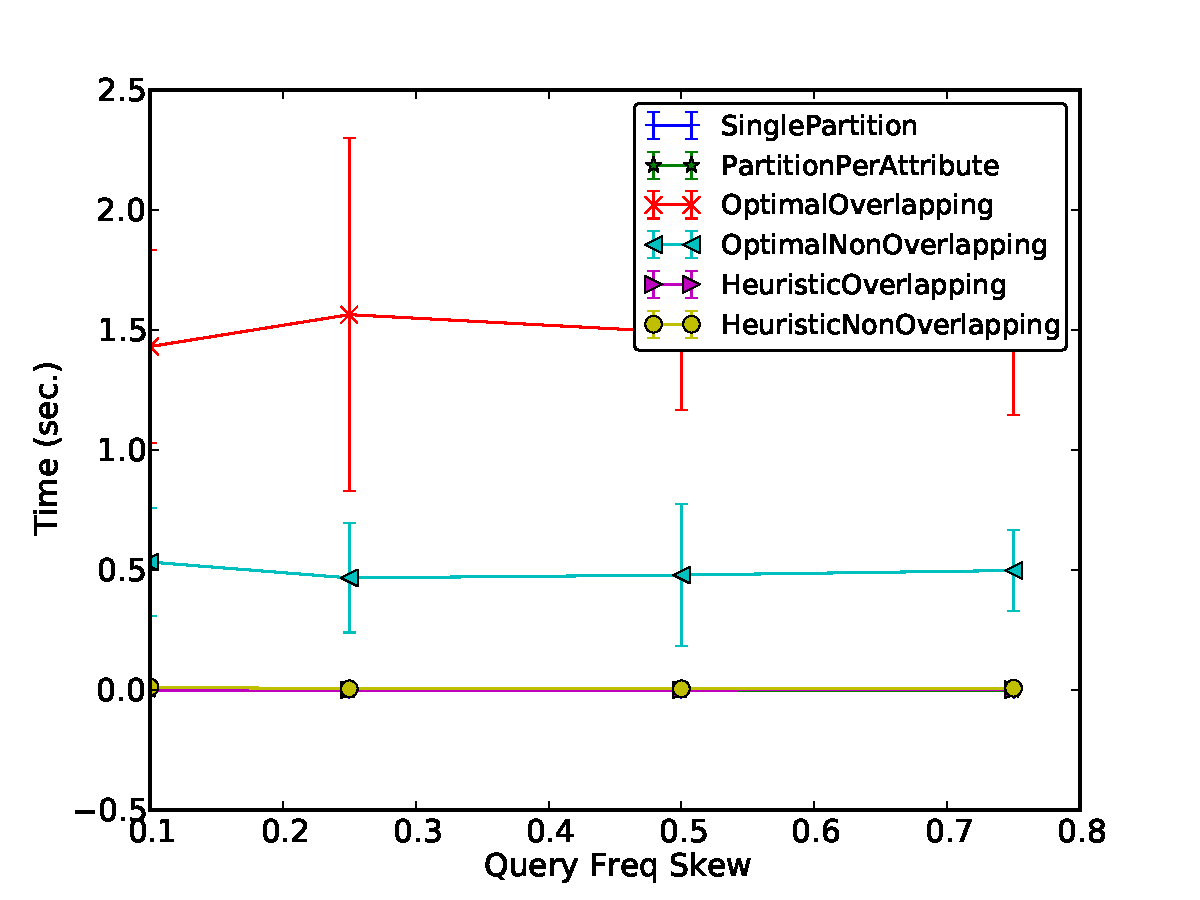
\includegraphics[width=0.9\columnwidth]{figures/RunningTimeVsQueryFreqSkew.pdf}}
\caption{RunningTimeVsQueryFreqSkew}
\end{figure}

\begin{figure}[ht]
\centerline{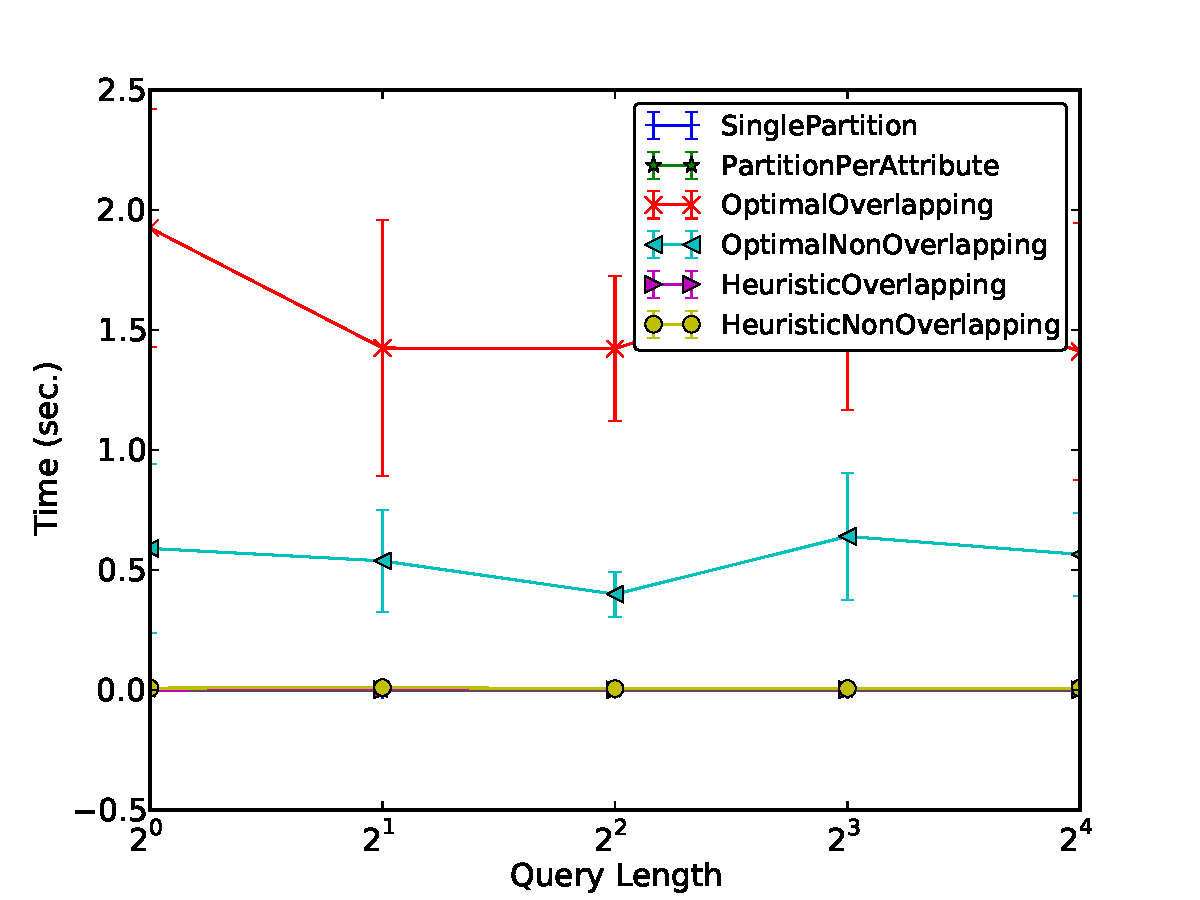
\includegraphics[width=0.9\columnwidth]{figures/RunningTimeVsQueryLength.pdf}}
\caption{RunningTimeVsQueryLength}
\end{figure}

\begin{figure}[ht]
\centerline{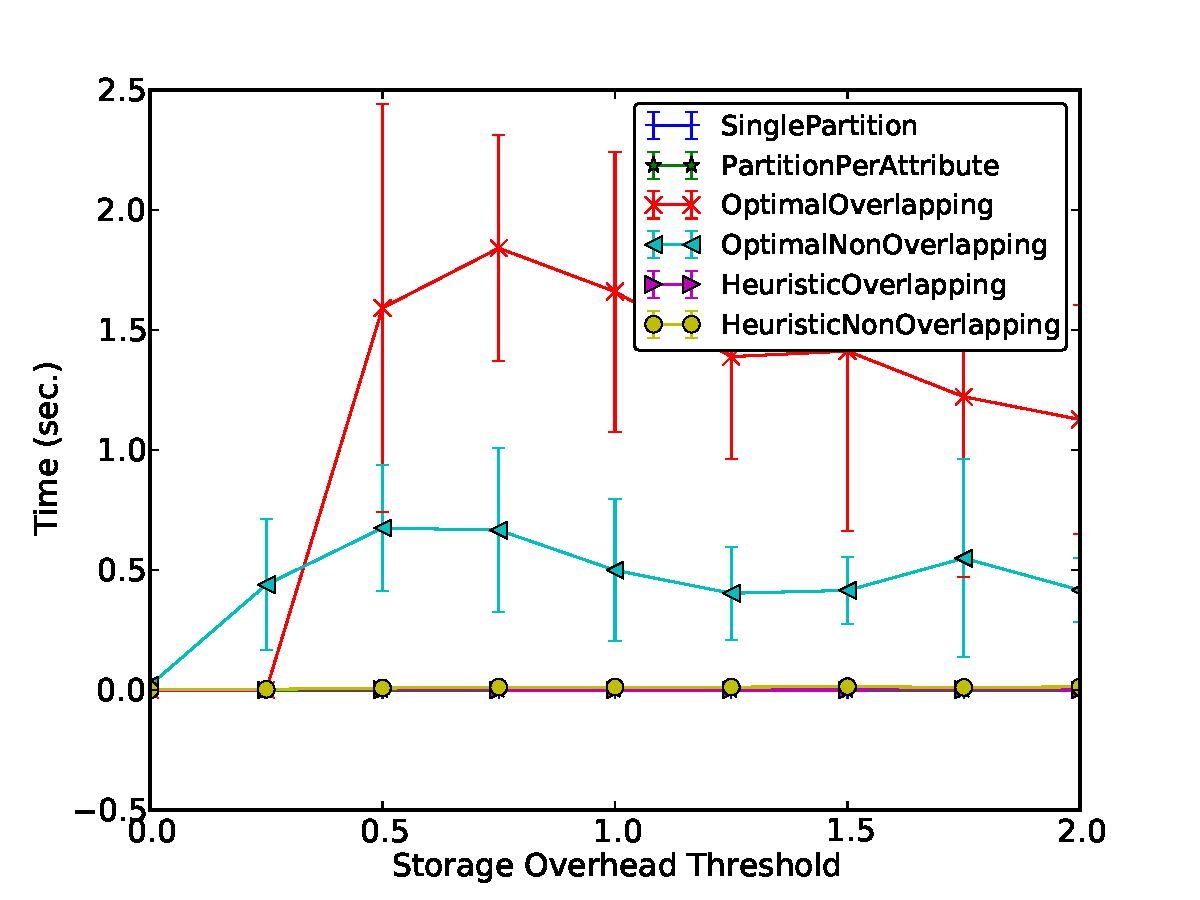
\includegraphics[width=0.9\columnwidth]{figures/RunningTimeVsStorageOverheadThreshold.pdf}}
\caption{RunningTimeVsStorageOverheadThreshold}
\end{figure}

%%%%%%%%%%%%%%%%%%%%%%%%%%%%%%%%%%%%%%%%%%%%%%

\subsection{Storage Overhead}

\begin{figure}[ht]
\centerline{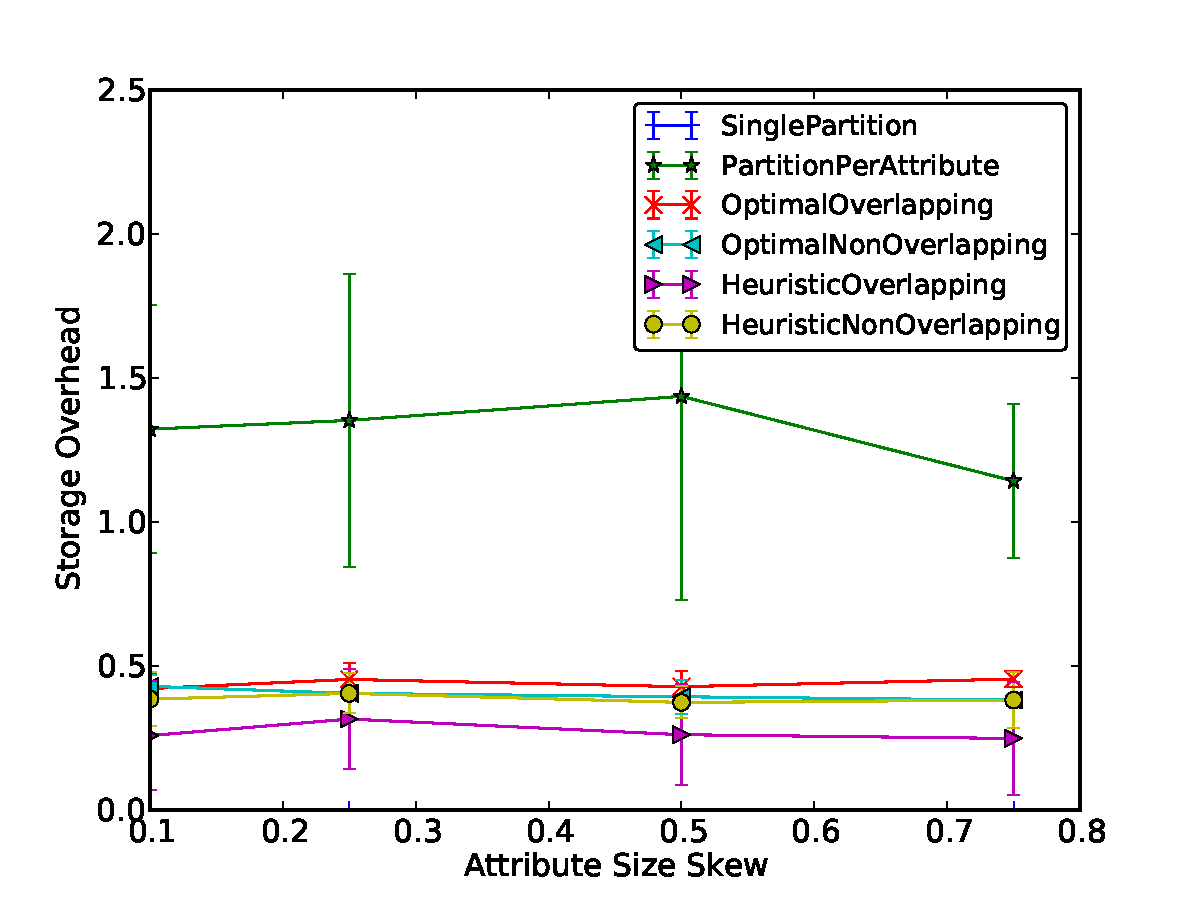
\includegraphics[width=0.9\columnwidth]{figures/StorageOverheadVsAttributeSizeSkew.pdf}}
\caption{StorageOverheadVsAttributeSizeSkew}
\end{figure}

\begin{figure}[ht]
\centerline{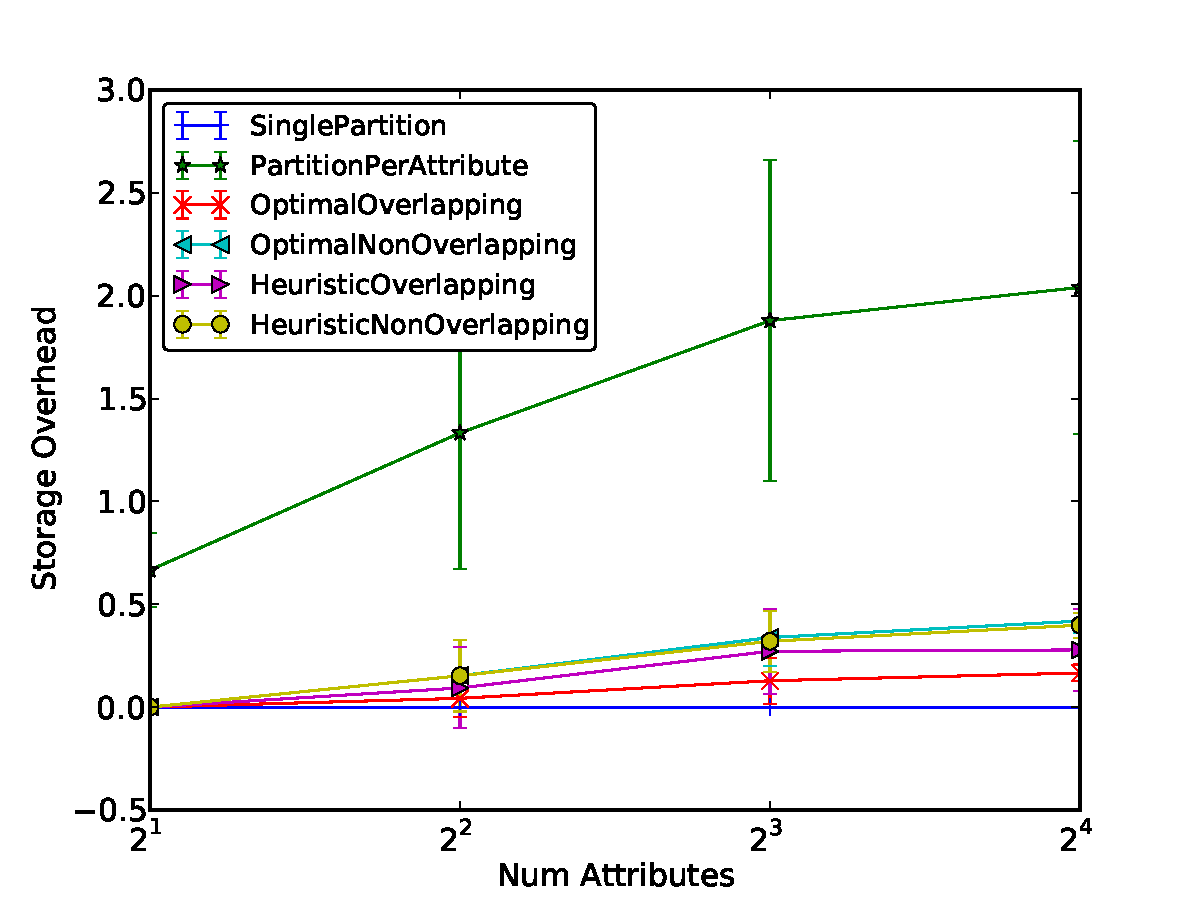
\includegraphics[width=0.9\columnwidth]{figures/StorageOverheadVsNumAttributes.pdf}}
\caption{StorageOverheadVsNumAttributes}
\end{figure}

\begin{figure}[ht]
\centerline{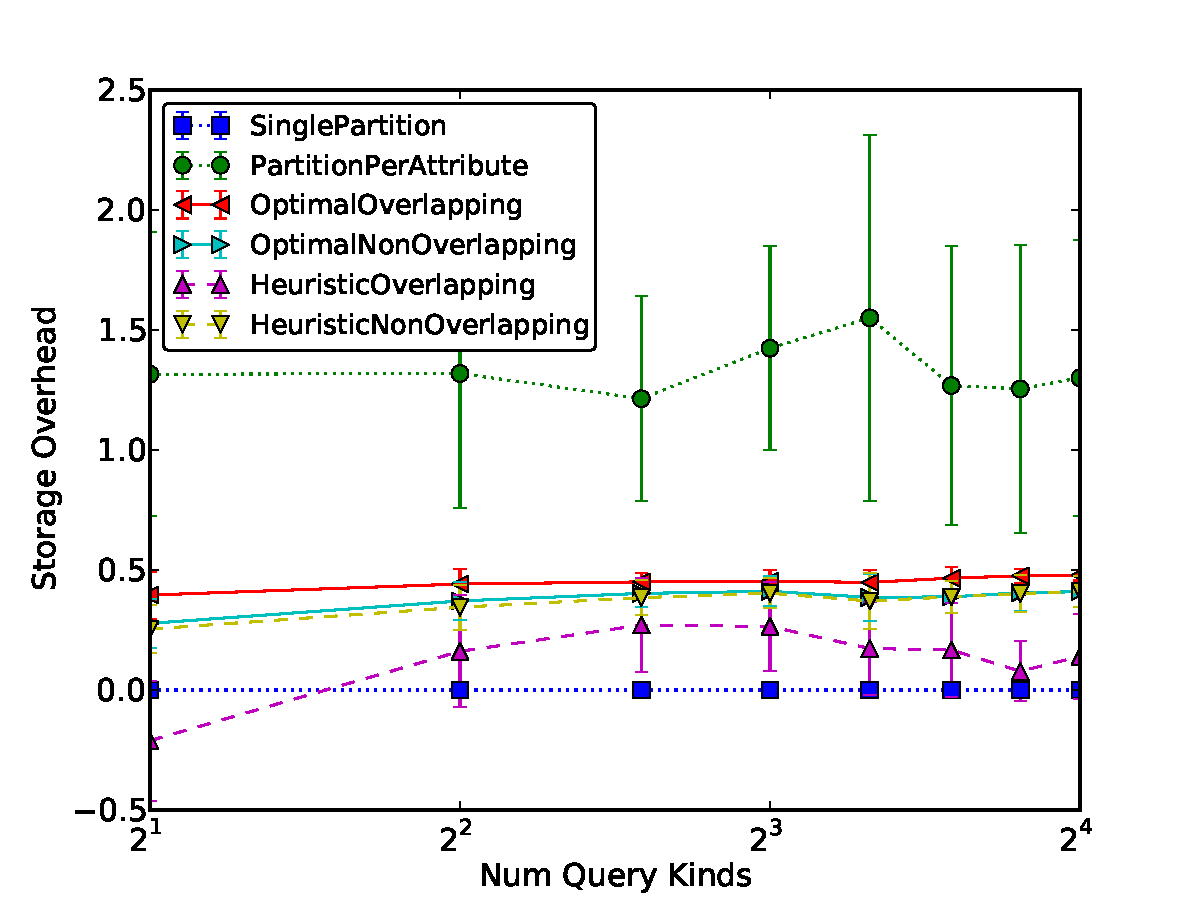
\includegraphics[width=0.9\columnwidth]{figures/StorageOverheadVsNumQueryKinds.pdf}}
\caption{StorageOverheadVsNumQueryKinds}
\end{figure}

\begin{figure}[ht]
\centerline{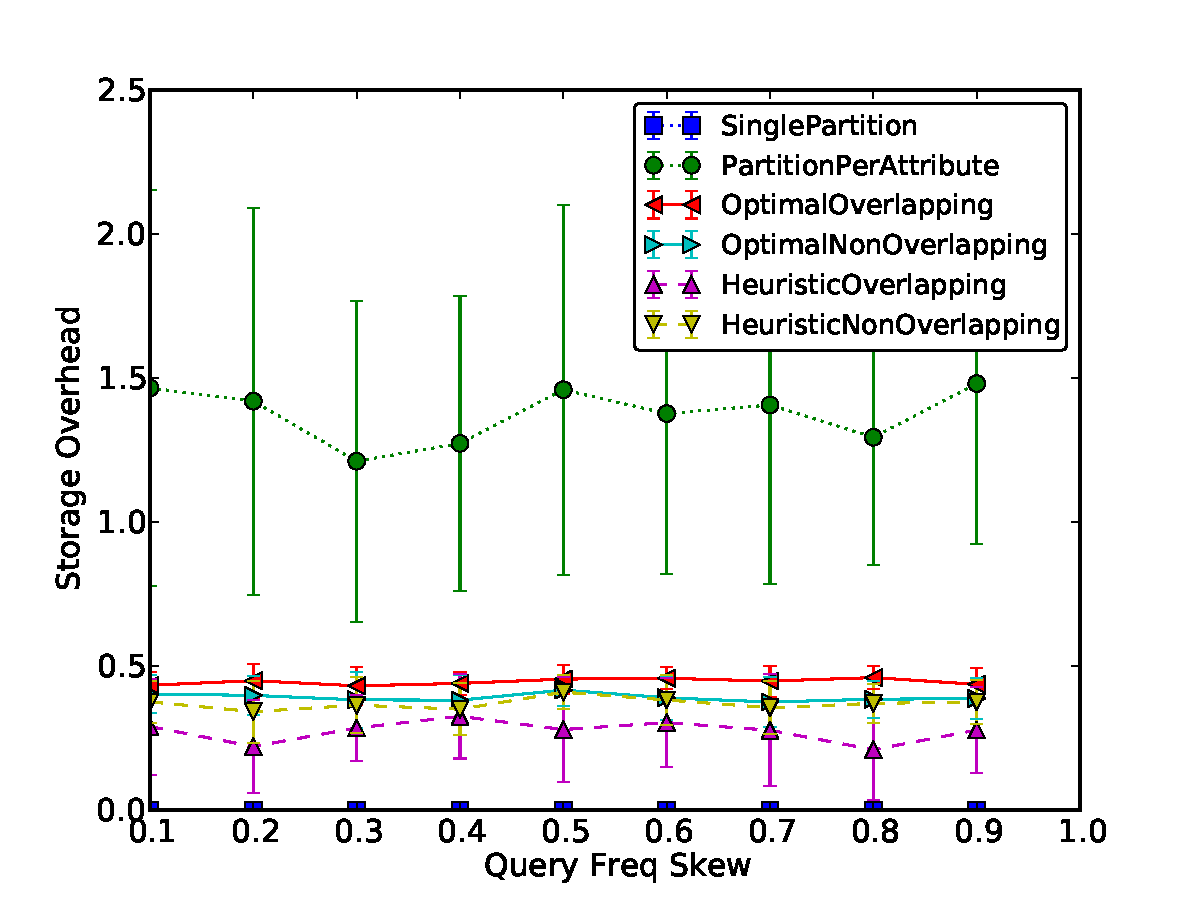
\includegraphics[width=0.9\columnwidth]{figures/StorageOverheadVsQueryFreqSkew.pdf}}
\caption{StorageOverheadVsQueryFreqSkew}
\end{figure}

\begin{figure}[ht]
\centerline{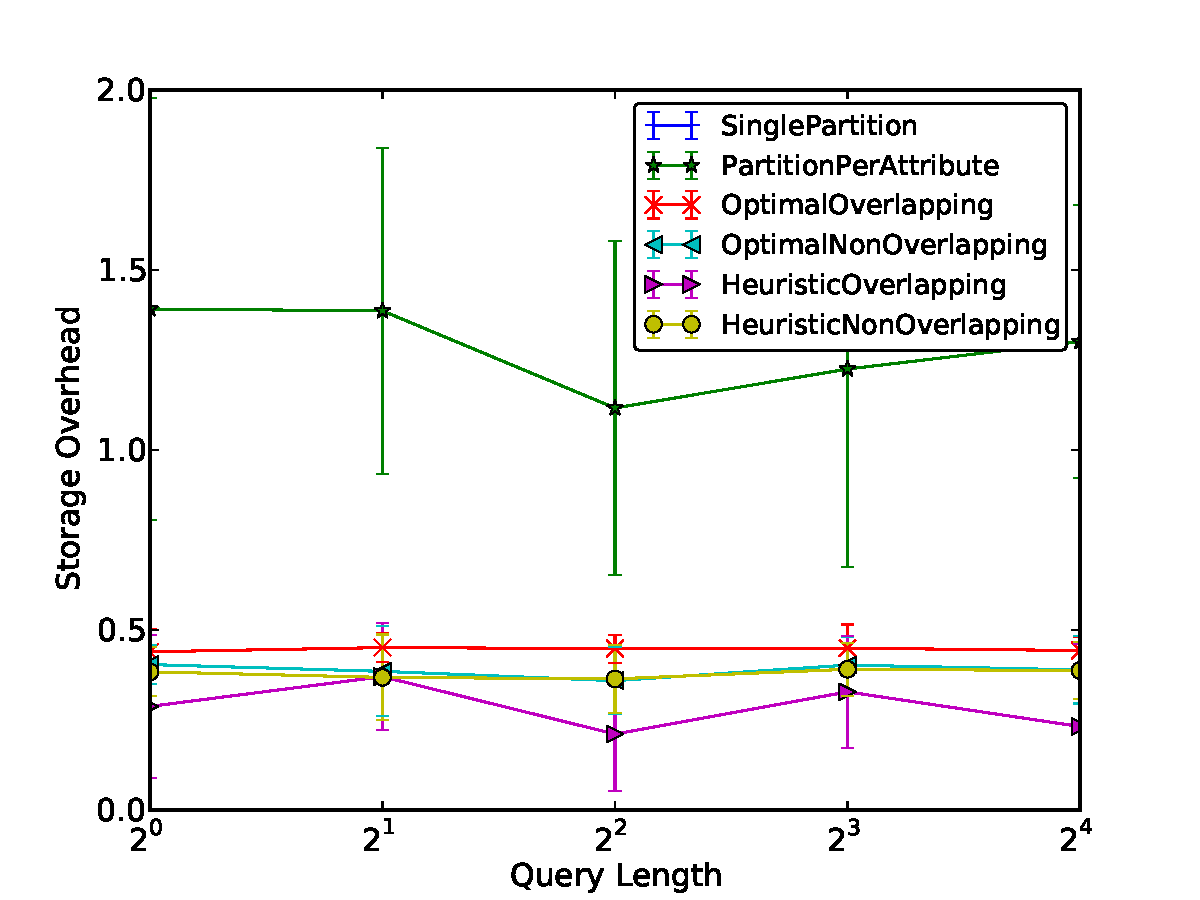
\includegraphics[width=0.9\columnwidth]{figures/StorageOverheadVsQueryLength.pdf}}
\caption{StorageOverheadVsQueryLength}
\end{figure}

% \begin{figure}[ht]
% \centerline{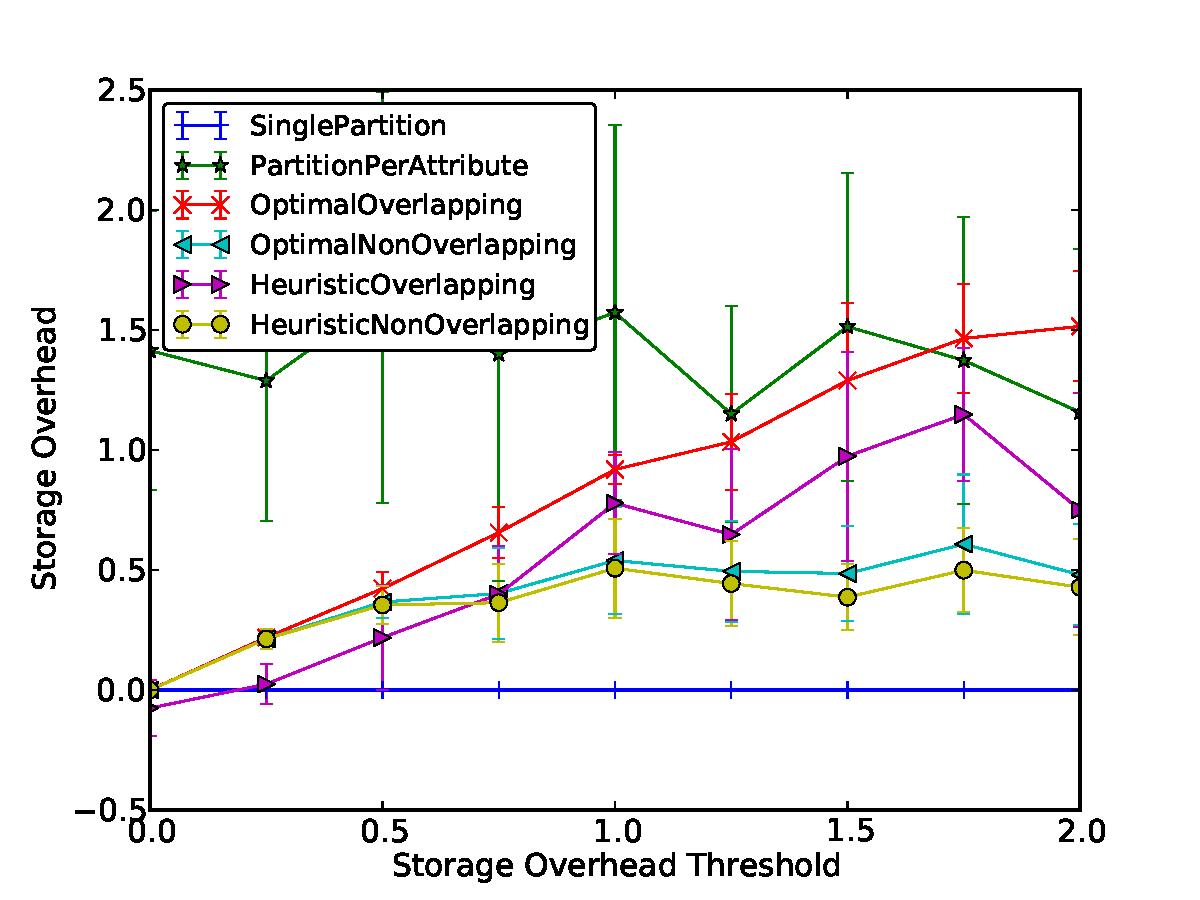
\includegraphics[width=0.9\columnwidth]{figures/StorageOverheadVsStorageOverheadThreshold.pdf}}
% \caption{StorageOverheadVsStorageOverheadThreshold}
% \end{figure}



%  \begin{figure*}[ht!]
%  \centerline{\begin{tabular}{c@{ }c@{ }c}
%  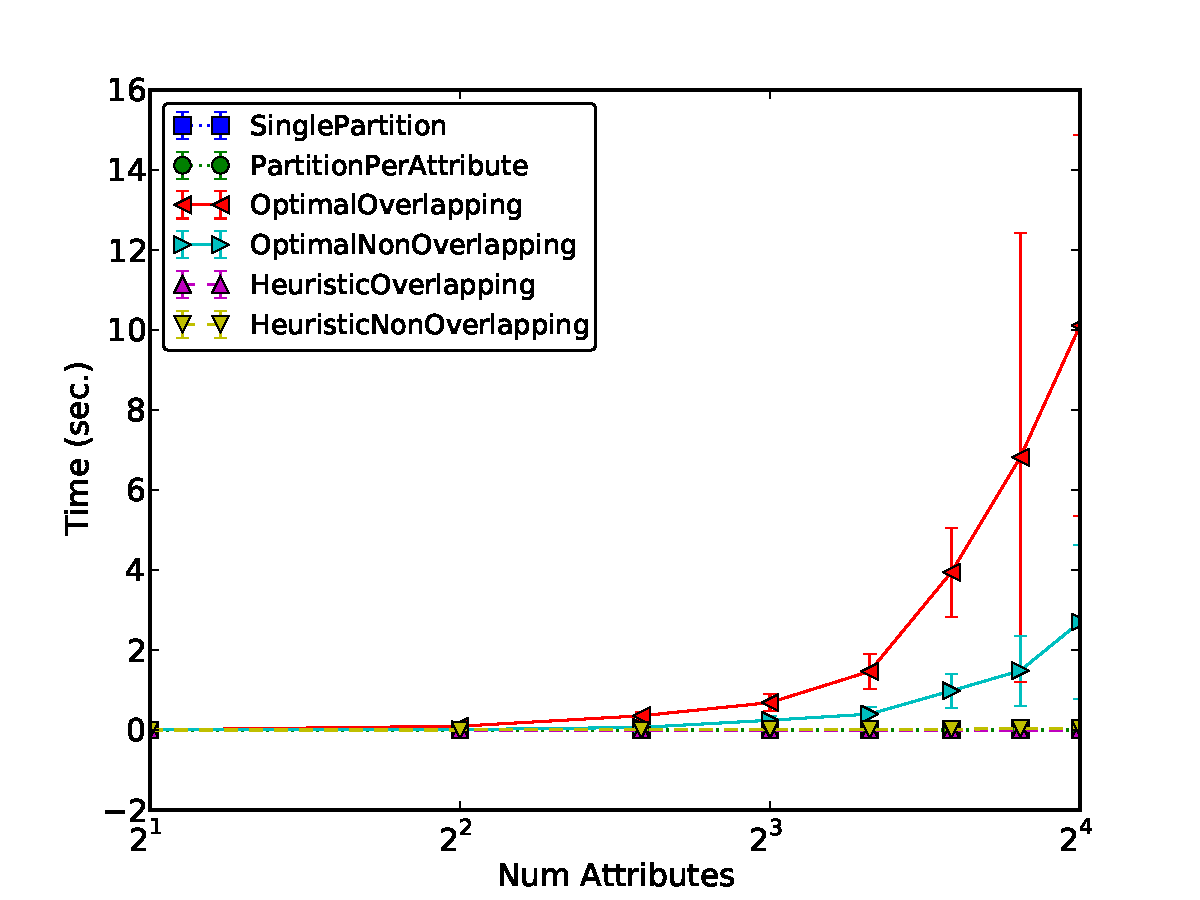
\includegraphics[width=0.33\textwidth]{figures/RunningTimeVsNumAttributes.pdf} &
%  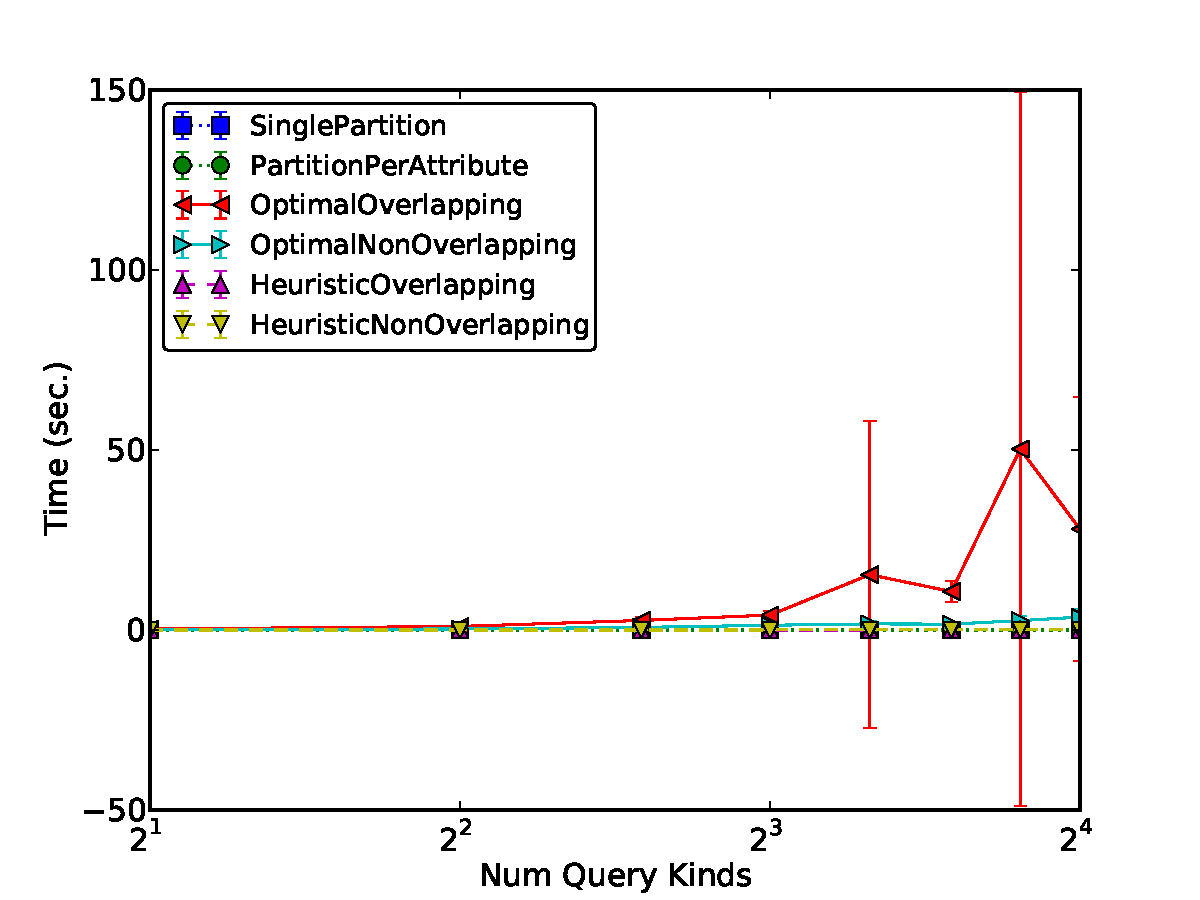
\includegraphics[width=0.33\textwidth]{figures/RunningTimeVsNumQueryKinds.pdf} &
%  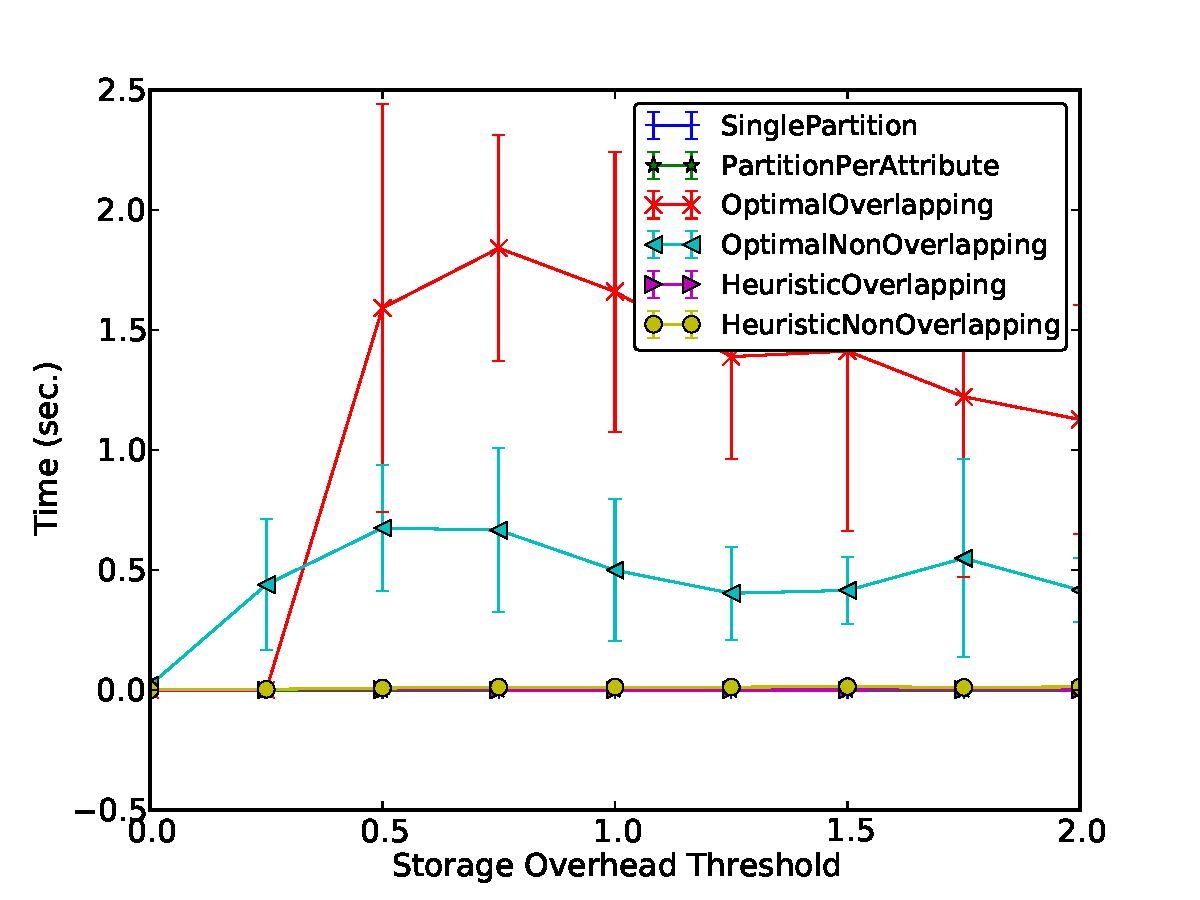
\includegraphics[width=0.33\textwidth]{figures/RunningTimeVsStorageOverheadThreshold.pdf}\\
%  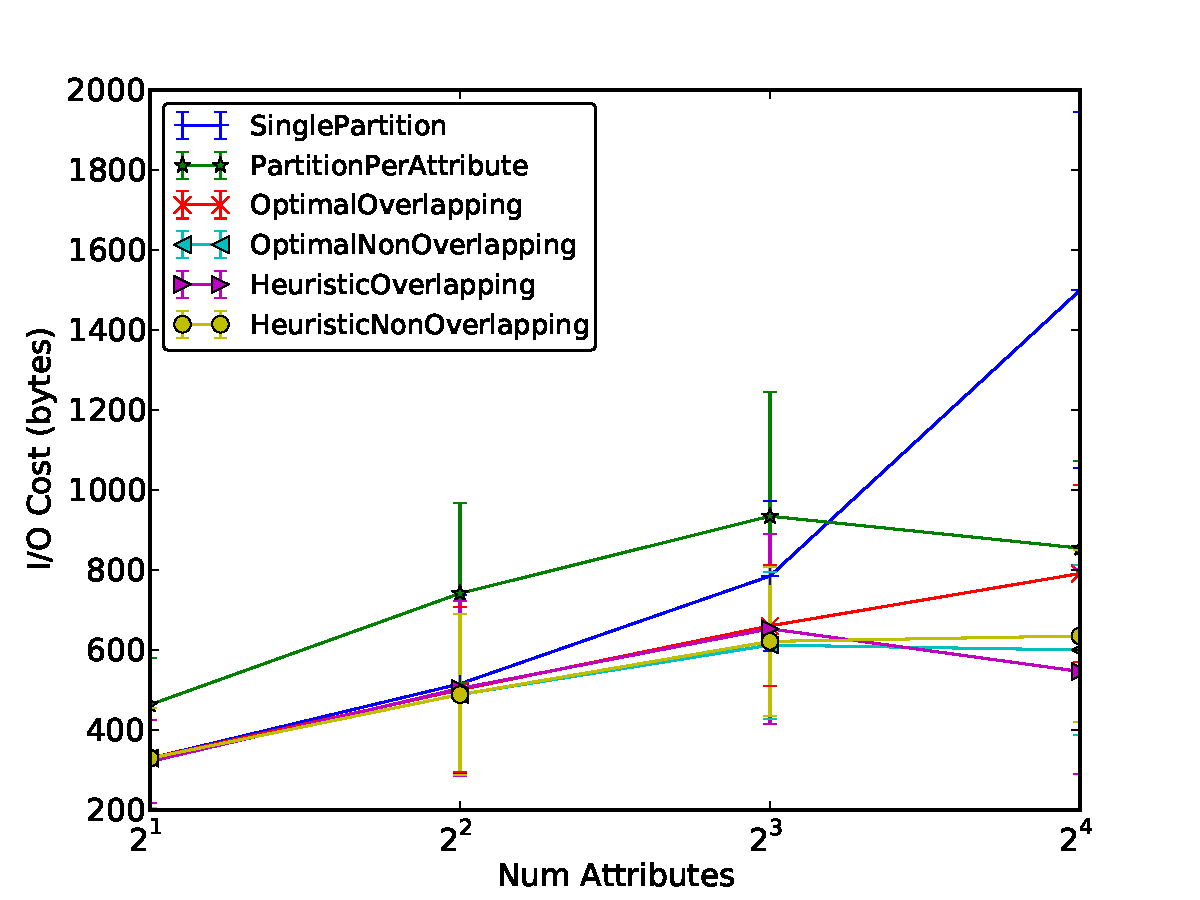
\includegraphics[width=0.33\textwidth]{figures/QueryIOVsNumAttributes.pdf} &
%  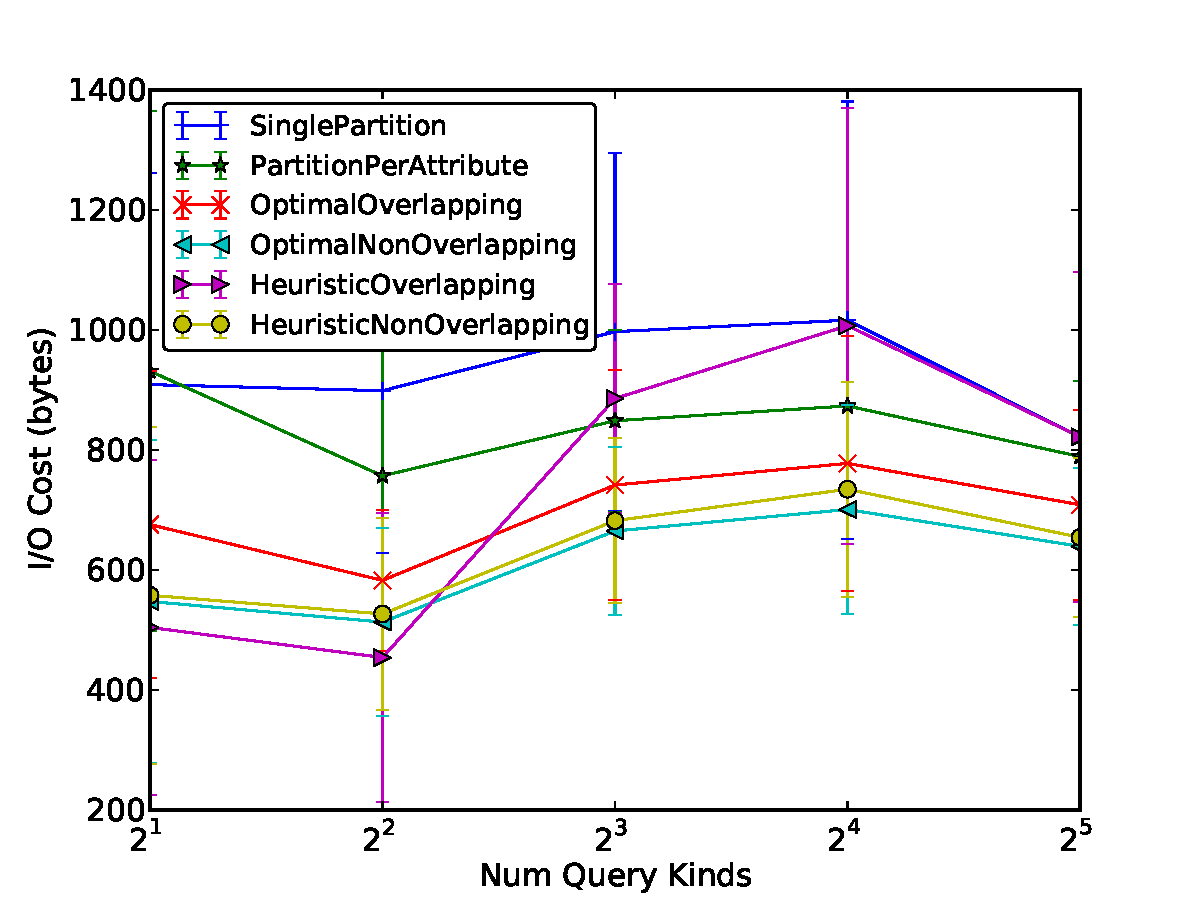
\includegraphics[width=0.33\textwidth]{figures/QueryIOVsNumQueryKinds.pdf} &
%  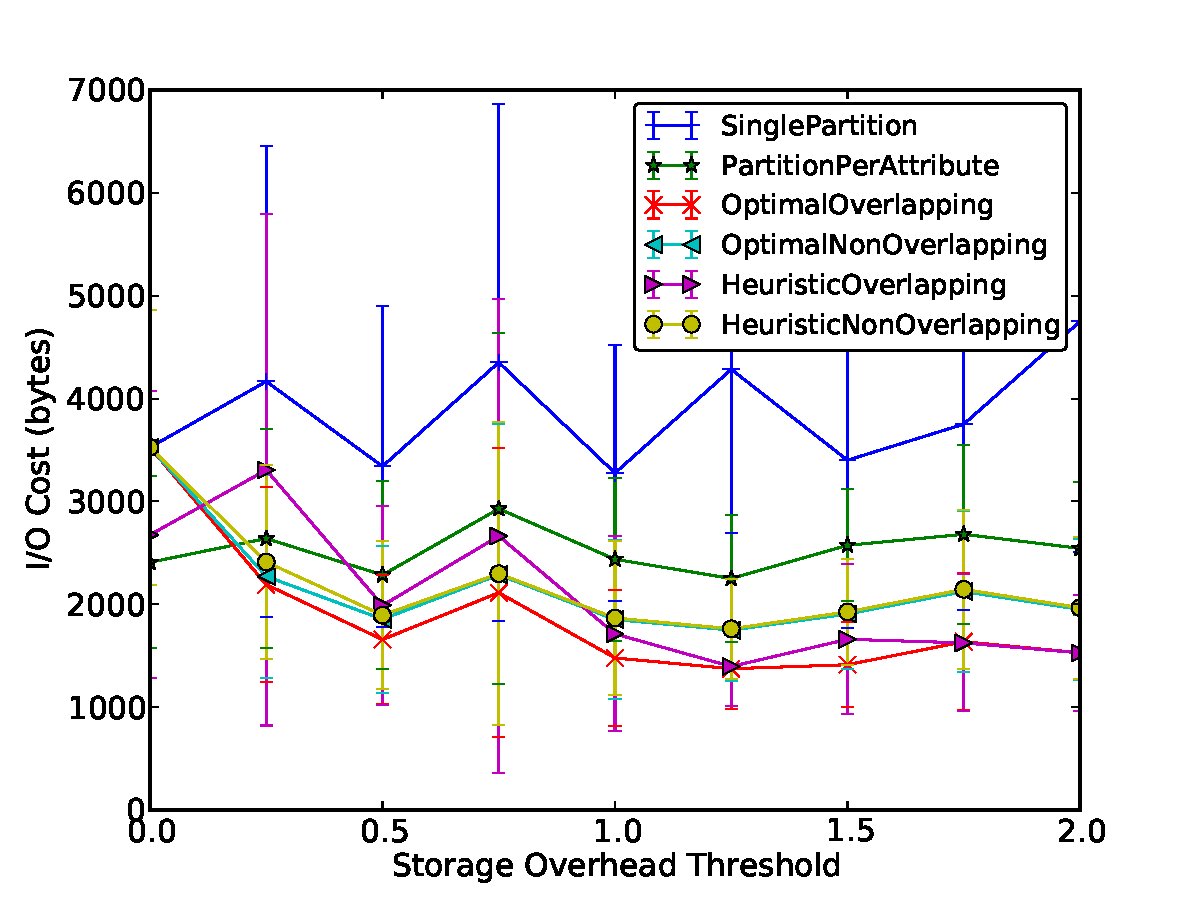
\includegraphics[width=0.33\textwidth]{figures/QueryIOVsStorageOverheadThreshold.pdf}\\
%  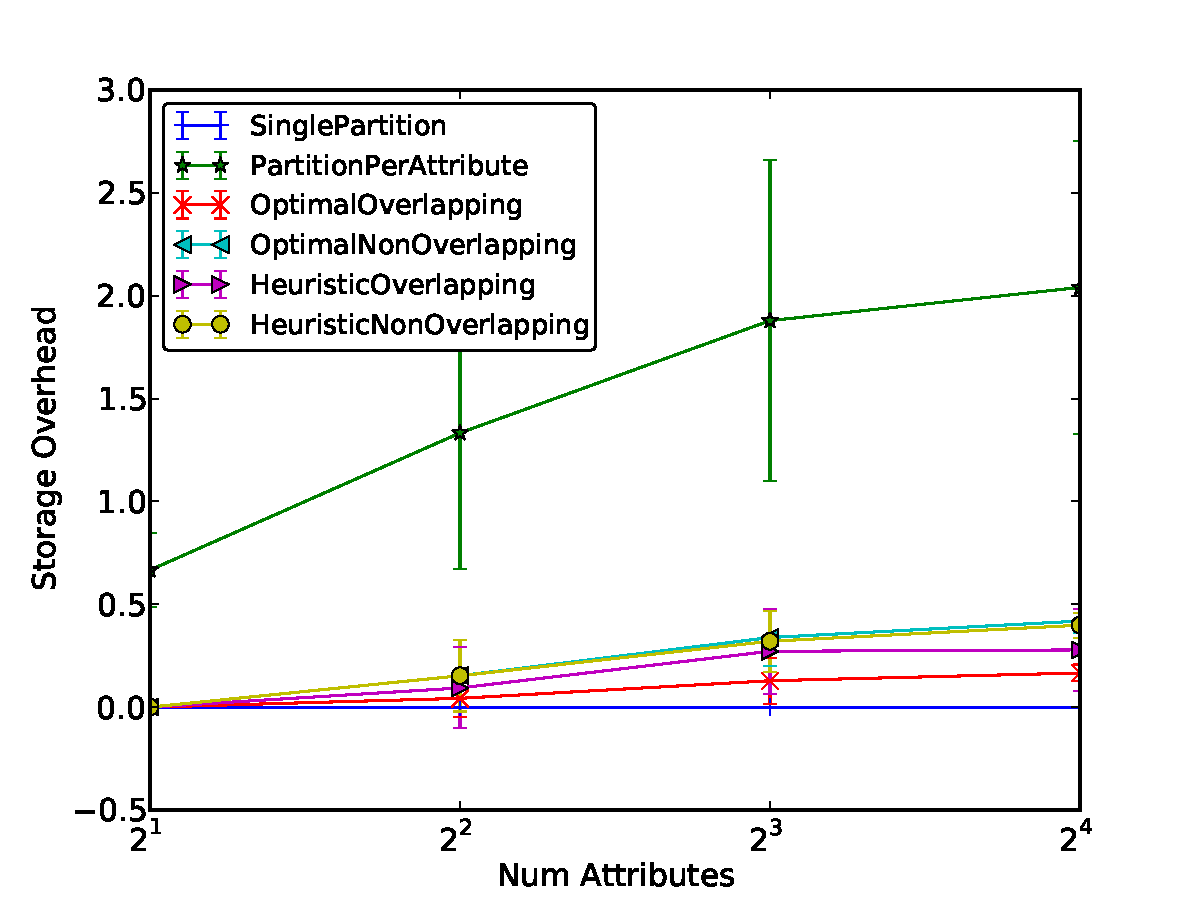
\includegraphics[width=0.33\textwidth]{figures/StorageOverheadVsNumAttributes.pdf} &
%  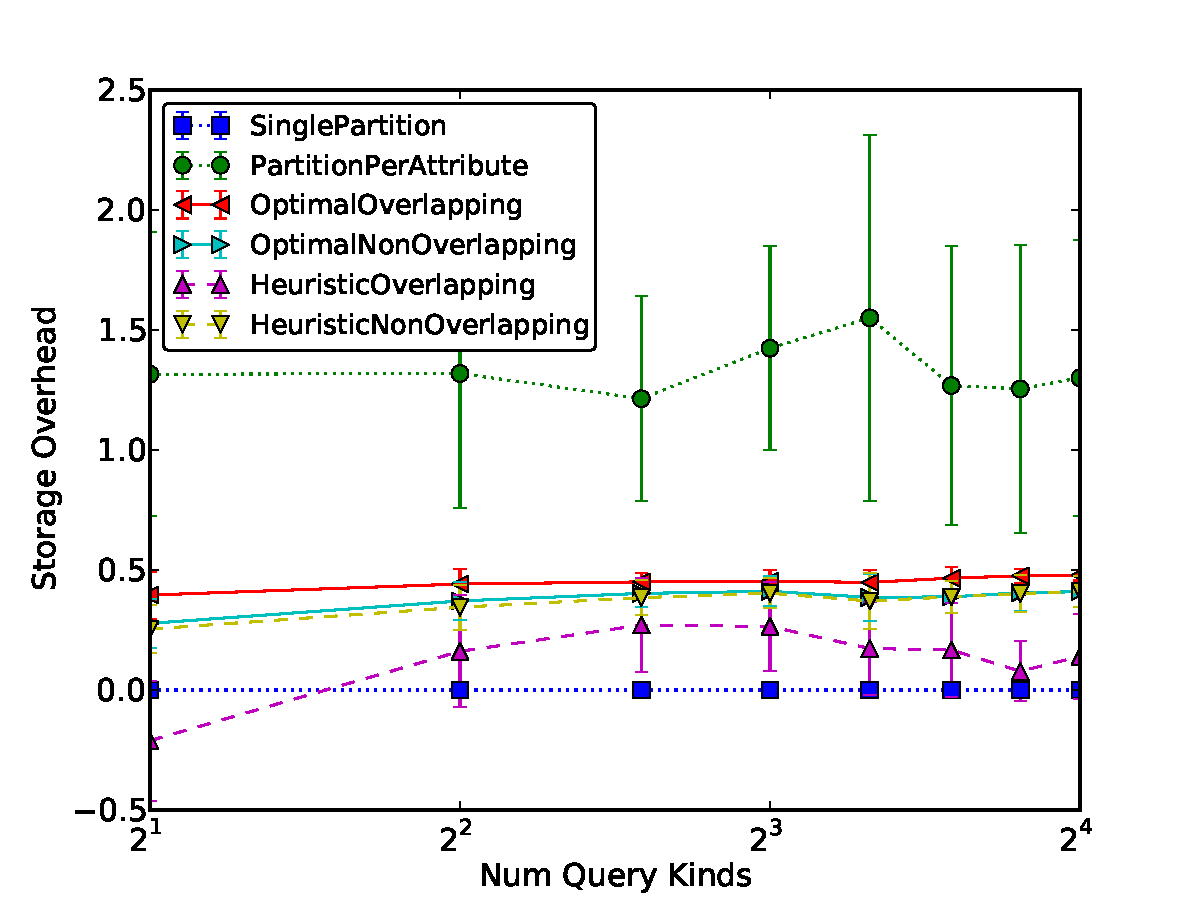
\includegraphics[width=0.33\textwidth]{figures/StorageOverheadVsNumQueryKinds.pdf} &
%  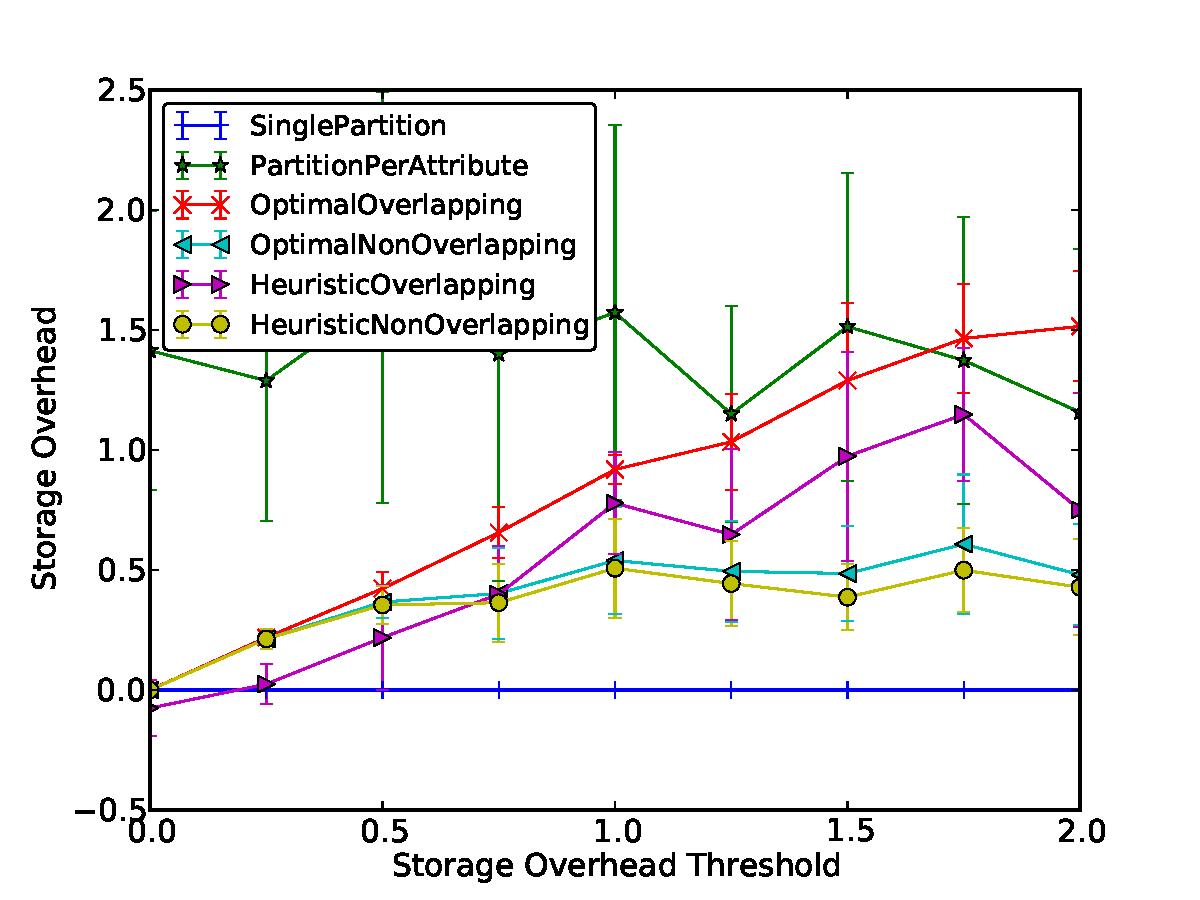
\includegraphics[width=0.33\textwidth]{figures/StorageOverheadVsStorageOverheadThreshold.pdf}\\
%  (a)Num Attributes & (b) NumQueryKind &
%  (c) StorageOverheadThreshold \\
%  \end{tabular}}
% \vspace*{1mm}
%  \caption{Running time, QueryIO, and StorageOverhead.}
%  \label{fig:results}
%  \end{figure*}



%%%%%%%%%%%%%%%%%%%%%%%%%%%%%%%%%%%%%%%%%%%%%%


\begin{verbatim}
1) RunningTimeVsNumAttributes:
  x axis: # attributes
  y axis: running time
  series: optimal-nov, optimal-ov, heuristic-nov, heuristic-ov

2) RunningTimeVsNumQueryKinds:
  x axis: num query kinds
  y axis: running time
  series: optimal-nov, optimal-ov, heuristic-nov, heuristic-ov

3) QueryIOVsNumAttributes:
  x axis: # attributes
  y axis: query IO
  series: optimal-nov, optimal-ov, heuristic-nov, heuristic-ov, single-block, per-attribute

4) StorageOverheadVsNumAttributes:
  x axis: # attributes
  y axis: storage overhead
  series: optimal-nov, optimal-ov, heuristic-nov, heuristic-ov, single-block, per-attribute
  
5) QueryIOVsStorageOverheadThreshold:
  x axis: query overhead threshold
  y axis: query IO
  series: optimal-nov, optimal-ov, heuristic-nov, heuristic-ov, single-block, per-attribute

6) StorageOverheadVsStorageOverheadThreshold:
  x axis: query overhead threshold
  y axis: storage overhead
  series: optimal-nov, optimal-ov, heuristic-nov, heuristic-ov, single-block, per-attribute

7) QueryIOVsNumQueryKinds:
  x axis: num query kinds
  y axis: query IO
  series: optimal-nov, optimal-ov, heuristic-nov, heuristic-ov, single-block, per-attribute

8) StorageOverheadVsNumQueryKinds:
  x axis: num query kinds
  y axis: storage overhead
  series: optimal-nov, optimal-ov, heuristic-nov, heuristic-ov, single-block, per-attribute

9) QueryIOVsAttributeSizeSkew:
  x axis: attribute size skew
  y axis: query IO
  series: optimal-nov, optimal-ov, heuristic-nov, heuristic-ov, single-block, per-attribute

10) StorageOverheadVsAttributeSizeSkew:
  x axis: attribute size skew
  y axis: storage overhead
  series: optimal-nov, optimal-ov, heuristic-nov, heuristic-ov, single-block, per-attribute

11) QueryIOVsQueryLength:
  x axis: mean query length
  y axis: query IO
  series: optimal-nov, optimal-ov, heuristic-nov, heuristic-ov, single-block, per-attribute

12) StorageOverheadVsQueryLength:
  x axis: mean query length
  y axis: storage overhead
  series: optimal-nov, optimal-ov, heuristic-nov, heuristic-ov, single-block, per-attribute

13) QueryIOVsQueryFreqSkew:
  x axis: query freq skew
  y axis: query IO
  series: optimal-nov, optimal-ov, heuristic-nov, heuristic-ov, single-block, per-attribute

14) StorageOverheadVsQueryFreqSkew:
  x axis: query freq skew
  y axis: storage overhead
  series: optimal-nov, optimal-ov, heuristic-nov, heuristic-ov, single-block, per-attribute
\end{verbatim}

